\documentclass[a4paper]{scrartcl}
\usepackage[cm]{fullpage}
\usepackage{amsmath, amssymb, esint}
\usepackage{siunitx}

\usepackage{tikz, pgfplots}
\tikzstyle{every node} = [align = center]
\pgfplotsset{
    compat = 1.9,
    potential/.style = { 
        axis lines = middle,
        grid = both,
        minor tick num = 3,
        every major grid/.style = {orange, opacity=0.5},
        clip = false,
        xmin = 0,
        ymin = 0,
        legend pos = outer north east
    },
    potential-scatter/.style = {
        only marks,
        error bars/.cd,
        x dir = both, y dir = both,
        x explicit, y explicit
    }
}

\begin{document}

\title{PHYS1241: Electrostatic Field Plotting}
\author{ \\ \\ }
\date{2015-08-20}
\maketitle

\section{Abstract}
The real electrostatic fields of some commonly idealised objects are measured and then compared with the ideal model of the objects. Most of the measurements fitted the ideal model, while the unfitted data was accounted for by end effects ignored by the ideal model.

\section{Introduction}
The electrostatic fields of various idealised shapes and arrangements of conductors are well known and often used in theoretical calculations. However, the fields in real-world situations are less well known, due to end effects, impurities and other non-ideal properties.

The purpose of this experiment is to examine the real-world electrostatic fields of planar representations of the often used idealised arrangements, long parallel plates, concentric cylinders and separated parallel cylinders, and also compare them to the theoretical expectations.

\section{Theoretical Problems}
\subsection{You have two parallel rectangular plates each with an area, \(A\). They are separated by a distance, \(d\). One plate has charge \(+Q\) placed on it and the other plate has charge \(-Q\).}
\subsubsection{Draw a Gaussian surface that you could use to calculate the electric field between the plates.}
\begin{center}
    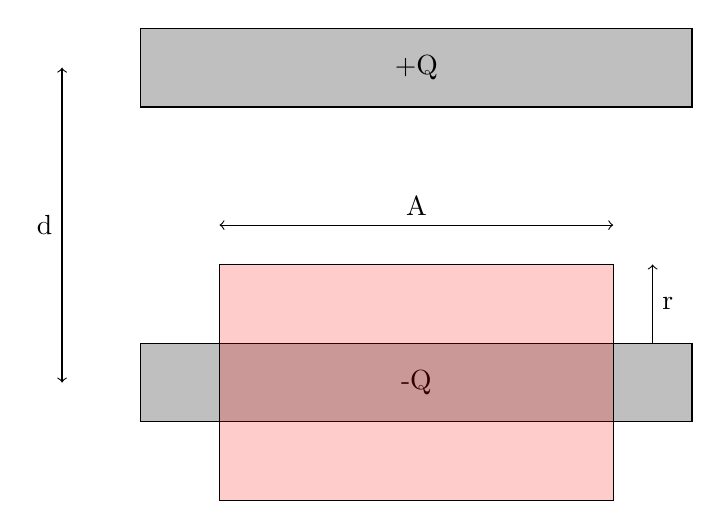
\begin{tikzpicture}
        \draw [<->] (-1, 0.5) -- (-1, 4.5) node [midway, left] {d};
        \draw [fill = white!50!gray] (0, 0) rectangle (7, 1) node [midway] {-Q};
        \draw [fill = white!50!gray] (0, 4) rectangle (7, 5) node [midway] {+Q};
        \draw [fill = red, fill opacity = .2] (1, -1) rectangle (6, 2);
        \draw [<->] (1, 2.5) -- (6, 2.5) node [midway, above] {A};
        \draw [->] (6.5, 1) -- (6.5, 2) node [midway, right] {r};
    \end{tikzpicture}
\end{center}

\subsubsection{Use the Gaussian surface to derive an expression for the electric field between the plates.}
\begin{align*}
    \frac{Q}{\varepsilon_0} \hat{r} &= \oiint_S \mathbf{E} \cdot \mathrm{d}\mathbf{A} = 2 A E \\
    E &= \frac{Q}{2 A \varepsilon_0} \hat{r} \\
    \therefore E_{net} &= E \bigg|_{Q=Q, \hat{r} = -1} + E \bigg|_{Q=-Q, \hat{r} = 1} \\
    &= -\frac{Q}{A \varepsilon_0}
\end{align*}

\subsubsection{Use your expression for the electric field to derive an expression for the potential difference between the \(-Q\) charged plate and a point, distance \(x\), from this plate along a line normal to the two plates.}
\begin{align*}
    \Delta V_P &= -\int_0^x E_{net} \cdot \mathrm{d}s \\
    &= -\left[ -\frac{Q}{A \varepsilon_0} s \right]_0^x \\
    &= \frac{Q x}{A \varepsilon_0}
\end{align*}

\subsubsection{A potential difference of \SI{12}{\volt} is maintained between two parallel rectangular plates. The distance between the two plates is \SI{60}{\milli\metre}. Plot a graph showing the variation of the potential difference between the two plates.}
\begin{align*}
    \Delta V_P \bigg|_{x = \SI{60}{\milli\metre}} &= \SI{12}{\volt} \\
    \therefore Q &= \frac{\SI{12}{\volt}}{\SI{60}{\milli\metre}} A \varepsilon_0 \\
    \therefore \Delta V_P &= \frac{\SI{12}{\volt}}{\SI{60}{\milli\metre}} x
\end{align*}
\begin{center}
    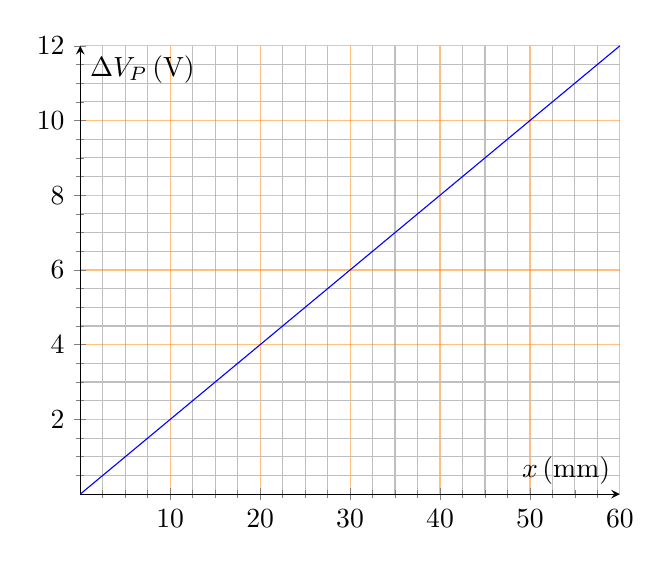
\begin{tikzpicture}
        \begin{axis}[
            potential,
            xlabel = \(x\,\mathrm{(mm)}\),
            ylabel = \(\Delta V_P\,\mathrm{(V)}\)
        ]
            \addplot +[no marks, domain = 0:60] {12 * x / 60};
        \end{axis}
    \end{tikzpicture}
\end{center}

\subsection{A Potential Difference of \SI{12}{\volt} is maintained between the cylinders of the capacitor described in Worked Example 1. The Potential of the inner cylinder is \SI{0}{\volt} and the outer cylinder is \SI{12}{\volt}. The cylinders have radii \(a = \SI{15}{\milli\metre}\) and \(b = \SI{100}{\milli\metre}\), respectively. The point \(P\) is a distance, \(r\), from the axis of the system, and between the cylinders.}
\subsubsection{Show that the potential difference, \(\Delta V_P\), between \(P\) and the inner cylinder is given by \(\Delta V_P = V \frac{\ln{r} - \ln{a}}{\ln{b} - \ln{a}} = 6.3 (\ln{r} - 2.7)\) where \(r\) is in \(\SI{}{\milli\metre}\).}
\begin{align*}
    \Delta V_P &= -\int_a^r \mathbf{E} \cdot \mathrm{d}\mathbf{r} \\
    &= \int_a^r \frac{Q}{2 \pi r l \varepsilon_0} \mathrm{d}r \\
    &= \frac{Q}{2 \pi l \varepsilon_0} \left[ \ln{r} \right]_a^r \\
    &= \frac{Q}{2 \pi l \varepsilon_0} \ln{\frac{r}{a}} \\
    \Delta V_P \bigg|_{r = b} &= V \\
    \therefore \frac{Q}{2 \pi l \varepsilon_0} &= \frac{V}{\ln{\frac{b}{a}}} \\
    \therefore \Delta V_P &= \frac{V \ln{\frac{r}{a}}}{\ln{\frac{b}{a}}} \\
    &= V \frac{\ln{r} - \ln{a}}{\ln{b} - \ln{a}} \\
    &= (\SI{12}{\volt})\frac{\ln{\frac{r}{\SI{15}{\milli\metre}}}}{\ln{\frac{\SI{100}{\milli\metre}}{\SI{15}{\milli\metre}}}} \\
    &\approx (\SI{6.3}{\volt}) (\ln{\frac{r}{\SI{}{\milli\metre}}} - 2.7) \\
    &\approx 6.3 (\ln{r} - 2.7) \text{ (Ignoring units)}
\end{align*}

\subsubsection{Plot a graph showing the variation of the potential at \(P\) as a function of its distance, \(r\), from the cylinder axis.}
\begin{center}
    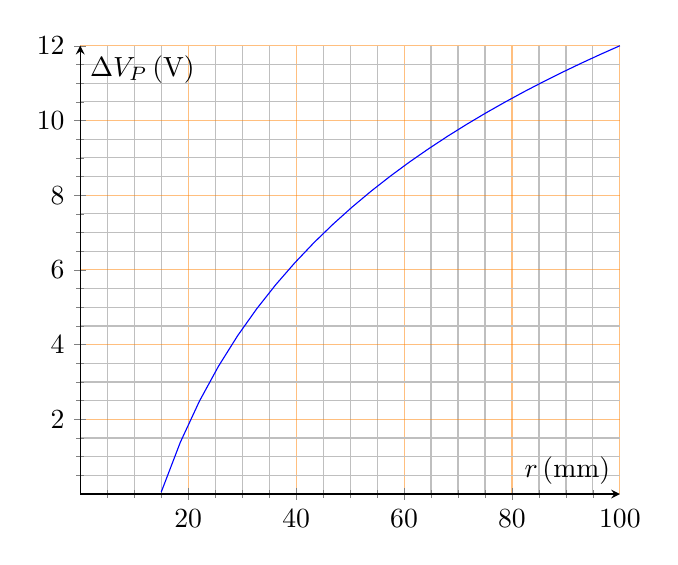
\begin{tikzpicture}
        \begin{axis}[
            potential,
            xlabel = \(r\,\mathrm{(mm)}\),
            ylabel = \(\Delta V_P\,\mathrm{(V)}\)
        ]
            \addplot +[no marks, domain = 15:100] {6.3 * (ln(x) - 2.7)};
        \end{axis}
    \end{tikzpicture}
\end{center}

\subsection{A capacitor like the one of Worked Example 2 has cylinders of radius \(a = \SI{10}{\milli\metre}\) and centre to centre separation \(d = \SI{140}{\milli\metre}\). It is charged so that it has \SI{0}{\volt} on the left hand cylinder and \SI{+12}{\volt} on the right hand cylinder.}
\subsubsection{Show that the Potential at point \(P\) which is a distance \(x\) from \(Q\) is given by \(\Delta V_P = 6 - 2.34 \ln{\frac{140 - x}{x}}\)}
\begin{align*}
    \Delta V_P &= -\int_a^x \mathbf{E} \cdot \mathrm{d}\mathbf{x} \\
    &= \int_a^x \frac{Q}{2 \pi l \varepsilon_0} \left( \frac{1}{x} + \frac{1}{d - x} \right) \mathrm{d}x \\
    &= \frac{Q}{2 \pi l \varepsilon_0} \left[ \ln{\frac{x}{d - x}} \right]_a^x \\
    &= \frac{Q}{2 \pi l \varepsilon_0} \ln{\frac{x (d - a)}{a (d - x)}} \\
    \Delta V_P \bigg|_{x = d - a} &= V \\
    \therefore \frac{Q}{2 \pi l \varepsilon_0} &= \frac{V}{\ln{\frac{(d - a)^2}{a^2}}} = \frac{V}{2 \ln{\frac{d - a}{a}}} \\
    \therefore \Delta V_P &= \frac{V \ln{\frac{x (d - a)}{a (d - x)}}}{2 \ln{\frac{d - a}{a}}} \\
    &= \frac{\SI{12}{\volt}}{2 \ln{\frac{\SI{130}{\milli\metre}}{\SI{10}{\milli\metre}}}} \ln{\frac{x (\SI{130}{\milli\metre})}{(\SI{1400}{\milli\metre\squared}) - x (\SI{10}{\milli\metre})}} \\
    &= -\frac{\SI{12}{\volt}}{2 \ln{13}} \ln{\frac{(\SI{140}{\milli\metre}) - x}{13 x}} \\
    &= -\frac{\SI{12}{\volt}}{2 \ln{13}} \left( \ln{\frac{(\SI{140}{\milli\metre}) - x}{x}} - \ln{13} \right) \\
    &= (\SI{6}{\volt}) - \frac{\SI{12}{\volt}}{2 \ln{13}} \ln{\frac{(\SI{140}{\milli\metre}) - x}{x}} \\
    &\approx 6 - 2.34 \ln{\frac{140 - x}{x}} \text{ (Ignoring units)}
\end{align*}

\subsubsection{Plot a graph showing the variation of the potential at \(P\) as a function of its distance, \(x\), from the cylinder axis.}
\begin{center}
    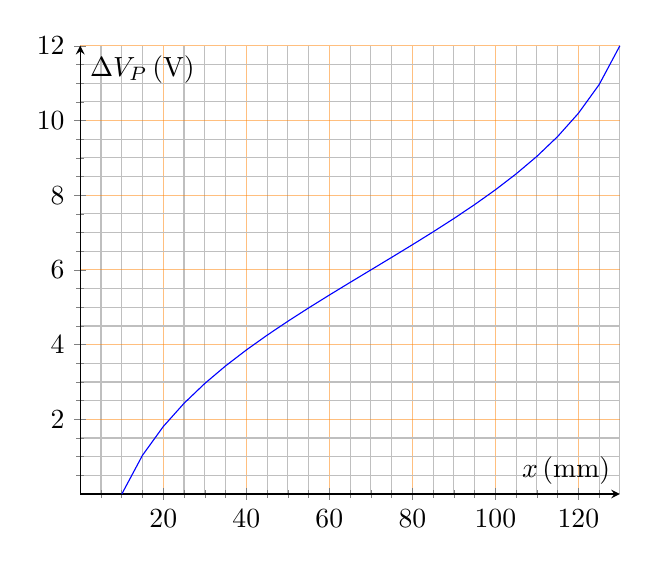
\begin{tikzpicture}
        \begin{axis}[
            potential,
            xlabel = \(x\,\mathrm{(mm)}\),
            ylabel = \(\Delta V_P\,\mathrm{(V)}\)
        ]
            \addplot +[no marks, domain = 10:130] {6 - 2.34 * ln((140 - x) / x)};
        \end{axis}
    \end{tikzpicture}
\end{center}

\section{Materials and Methods}
Please refer to pages 64 to 68 inclusive in the PHYS1241 laboratory manual for the base materials and methods used.

Of the multimeter and electrometer provided, the electrometer was chosen for primary use due to its fast analogue readout and very high impedance, both contributing to a more accurate measurement.

Measurement was taken by finding a point on the paper corresponding to the target voltage with the probe, and then while watching the electrometer, "walking" the probe in the expected direction of an equipotential contour while simultaneously marking the paper, and adjusting the position when the reading started to change by more than \SI{\pm 0.1}{\volt}. The line was then smoothed.

Uncertainty was estimated by both examining how much the voltage measurement differed by when retracing the previously found equipotential markings, and how far the voltage measurement changed by merely moving the position of the handle. This was determined to be within \SI{\pm 0.3}{\volt} for each arrangement.

\section{Results}
The two reference voltages were \SI{0.00 \pm 0.01}{\volt} and \SI{12.00 \pm 0.01}{\volt}, while the remaining voltage measurements were all within \SI{\pm 0.5}{\volt}. For clarity, these uncertainties are not shown on the equipotential plots.

Unfortunately, due to the low number of data points gathered, goodness of fit to the ideal model can only be eyeballed rather than statistically calculated.

\subsection{Long Parallel Plates}
\begin{figure}
    \centering
    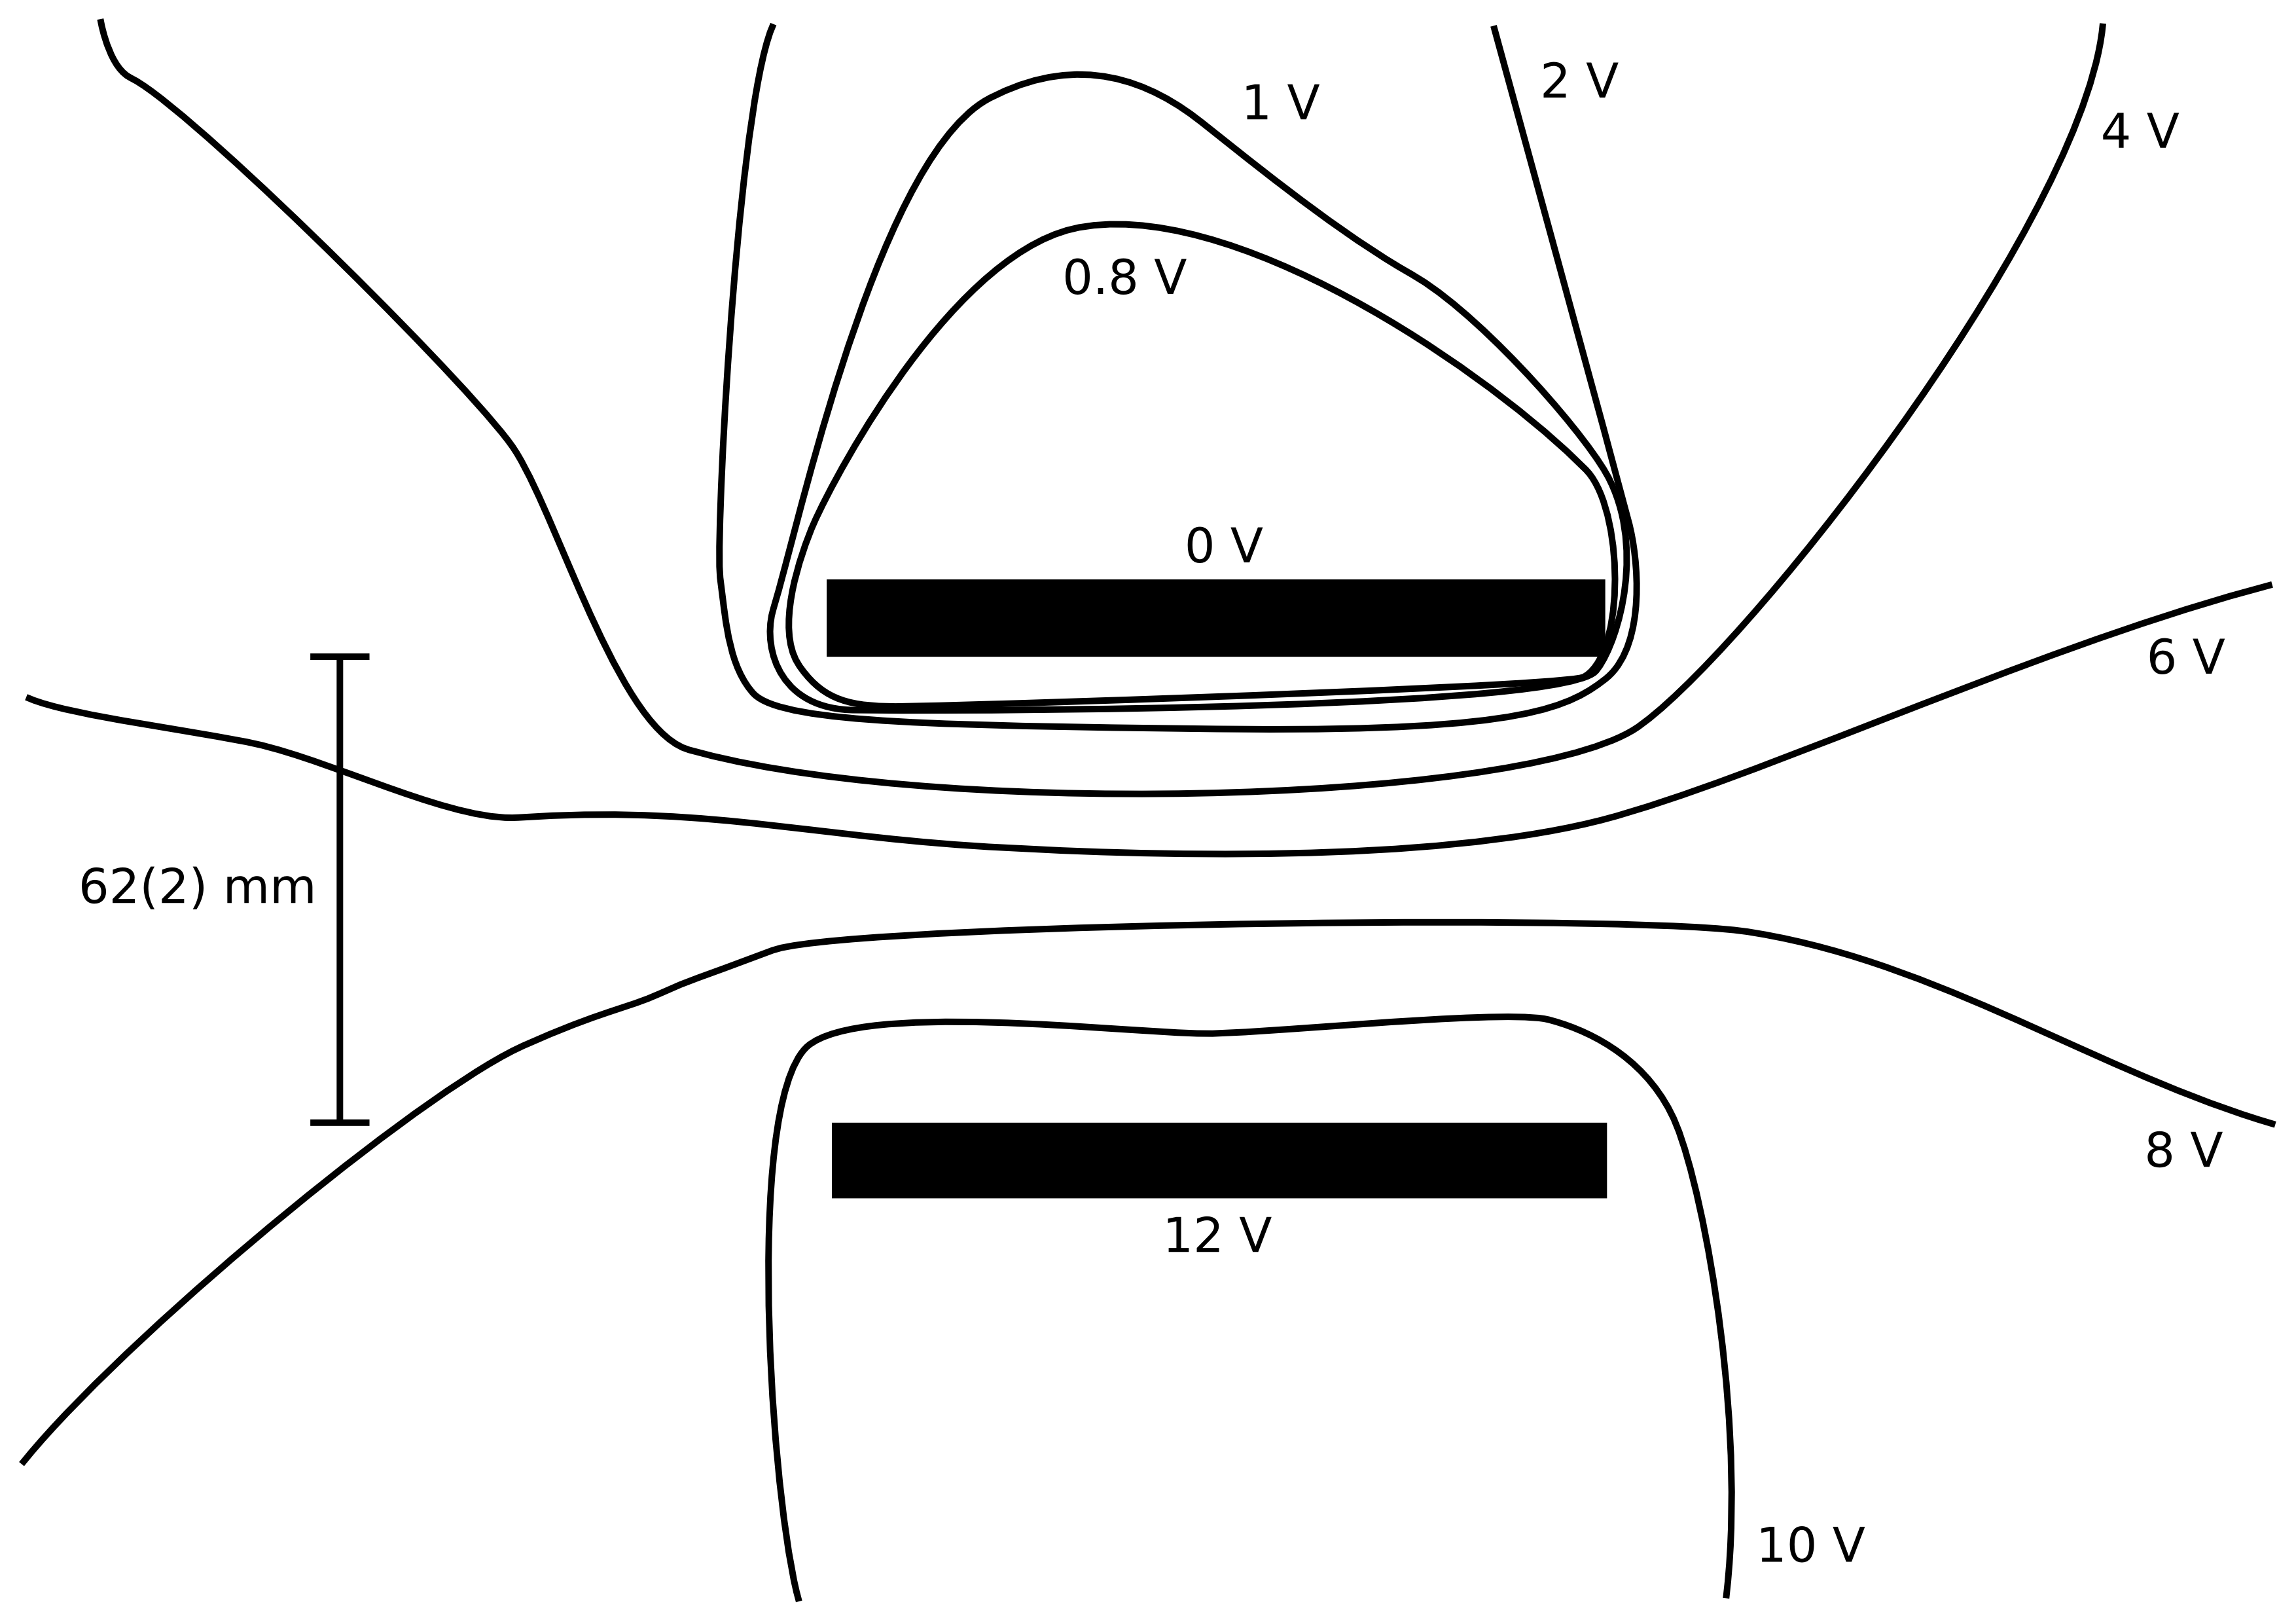
\includegraphics[width = 15cm]{lab2_parallel_plates.png}
    \caption{Equipotential lines for the two plates}
    \label{fig:parallel_plates}
\end{figure}
\begin{figure}
    \centering
    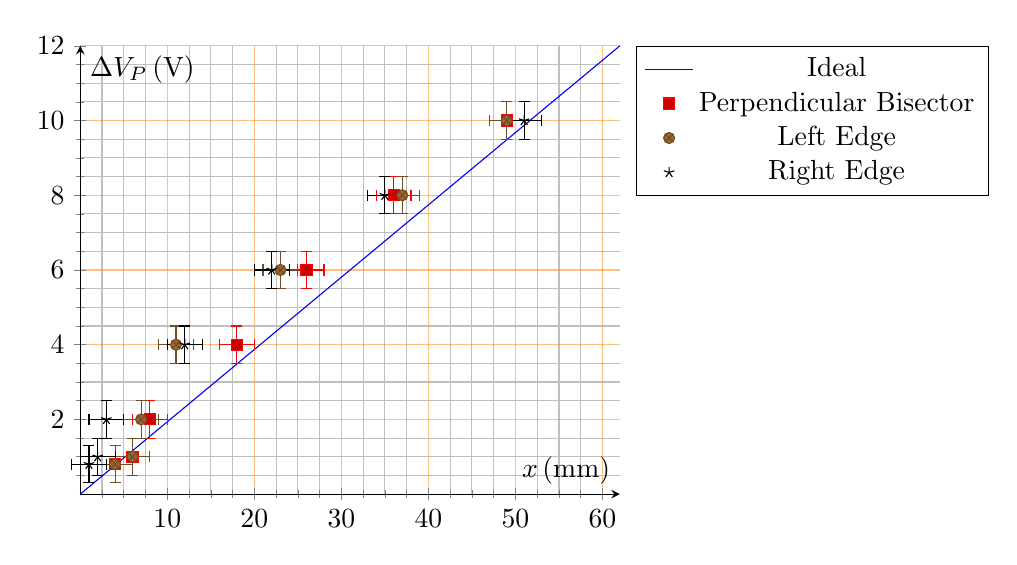
\begin{tikzpicture}
        \begin{axis}[
            potential,
            xlabel = \(x\,\mathrm{(mm)}\),
            ylabel = \(\Delta V_P\,\mathrm{(V)}\)
        ]
            \addplot +[no marks, domain = 0:62] {12 * x / 62};
            \addlegendentry{Ideal}
            
            \addplot +[potential-scatter] table [
                x error = xerror,
                y error = yerror
            ] {
                x   y   xerror  yerror
                4   0.8 2       0.5
                6   1   2       0.5
                8   2   2       0.5
                18  4   2       0.5
                26  6   2       0.5
                36  8   2       0.5
                49  10  2       0.5
            };
            \addlegendentry{Perpendicular Bisector}
                                                
            \addplot +[potential-scatter] table [
                x error = xerror,
                y error = yerror
            ] {
                x   y   xerror  yerror
                4   0.8 2       0.5
                6   1   2       0.5
                7   2   2       0.5
                11  4   2       0.5
                23  6   2       0.5
                37  8   2       0.5
                49  10  2       0.5
            };
            \addlegendentry{Left Edge}
                                                
            \addplot +[potential-scatter] table [
                x error = xerror,
                y error = yerror
            ] {
                x   y   xerror  yerror
                1   0.8 2       0.5
                2   1   2       0.5
                3   2   2       0.5
                12  4   2       0.5
                22  6   2       0.5
                35  8   2       0.5
                51  10  2       0.5
            };
            \addlegendentry{Right Edge}
        \end{axis}
    \end{tikzpicture}
    \caption{Voltage difference between the plates}
    \label{fig:parallel_plates_voltage}
\end{figure}

Figure \ref{fig:parallel_plates} shows the equipotential contours recorded. Figure \ref{fig:parallel_plates_voltage} shows the measured voltage at certain distances perpendicular to the plates.

The perpendicular bisector's results mostly fits the ideal model within the error margin, but two data points are outside the error margin. The data recorded at the edges starts bulging away from the ideal model non-linearly.

The multimeter was also used briefly to compare the results with the electrometer measurements. While it returned measurements within the error margin between the plates, it gave up to a \SI{\pm 3}{\volt} difference in reading at areas further from the plates.

\subsection{Concentric Cylinders}
\begin{figure}
    \centering
    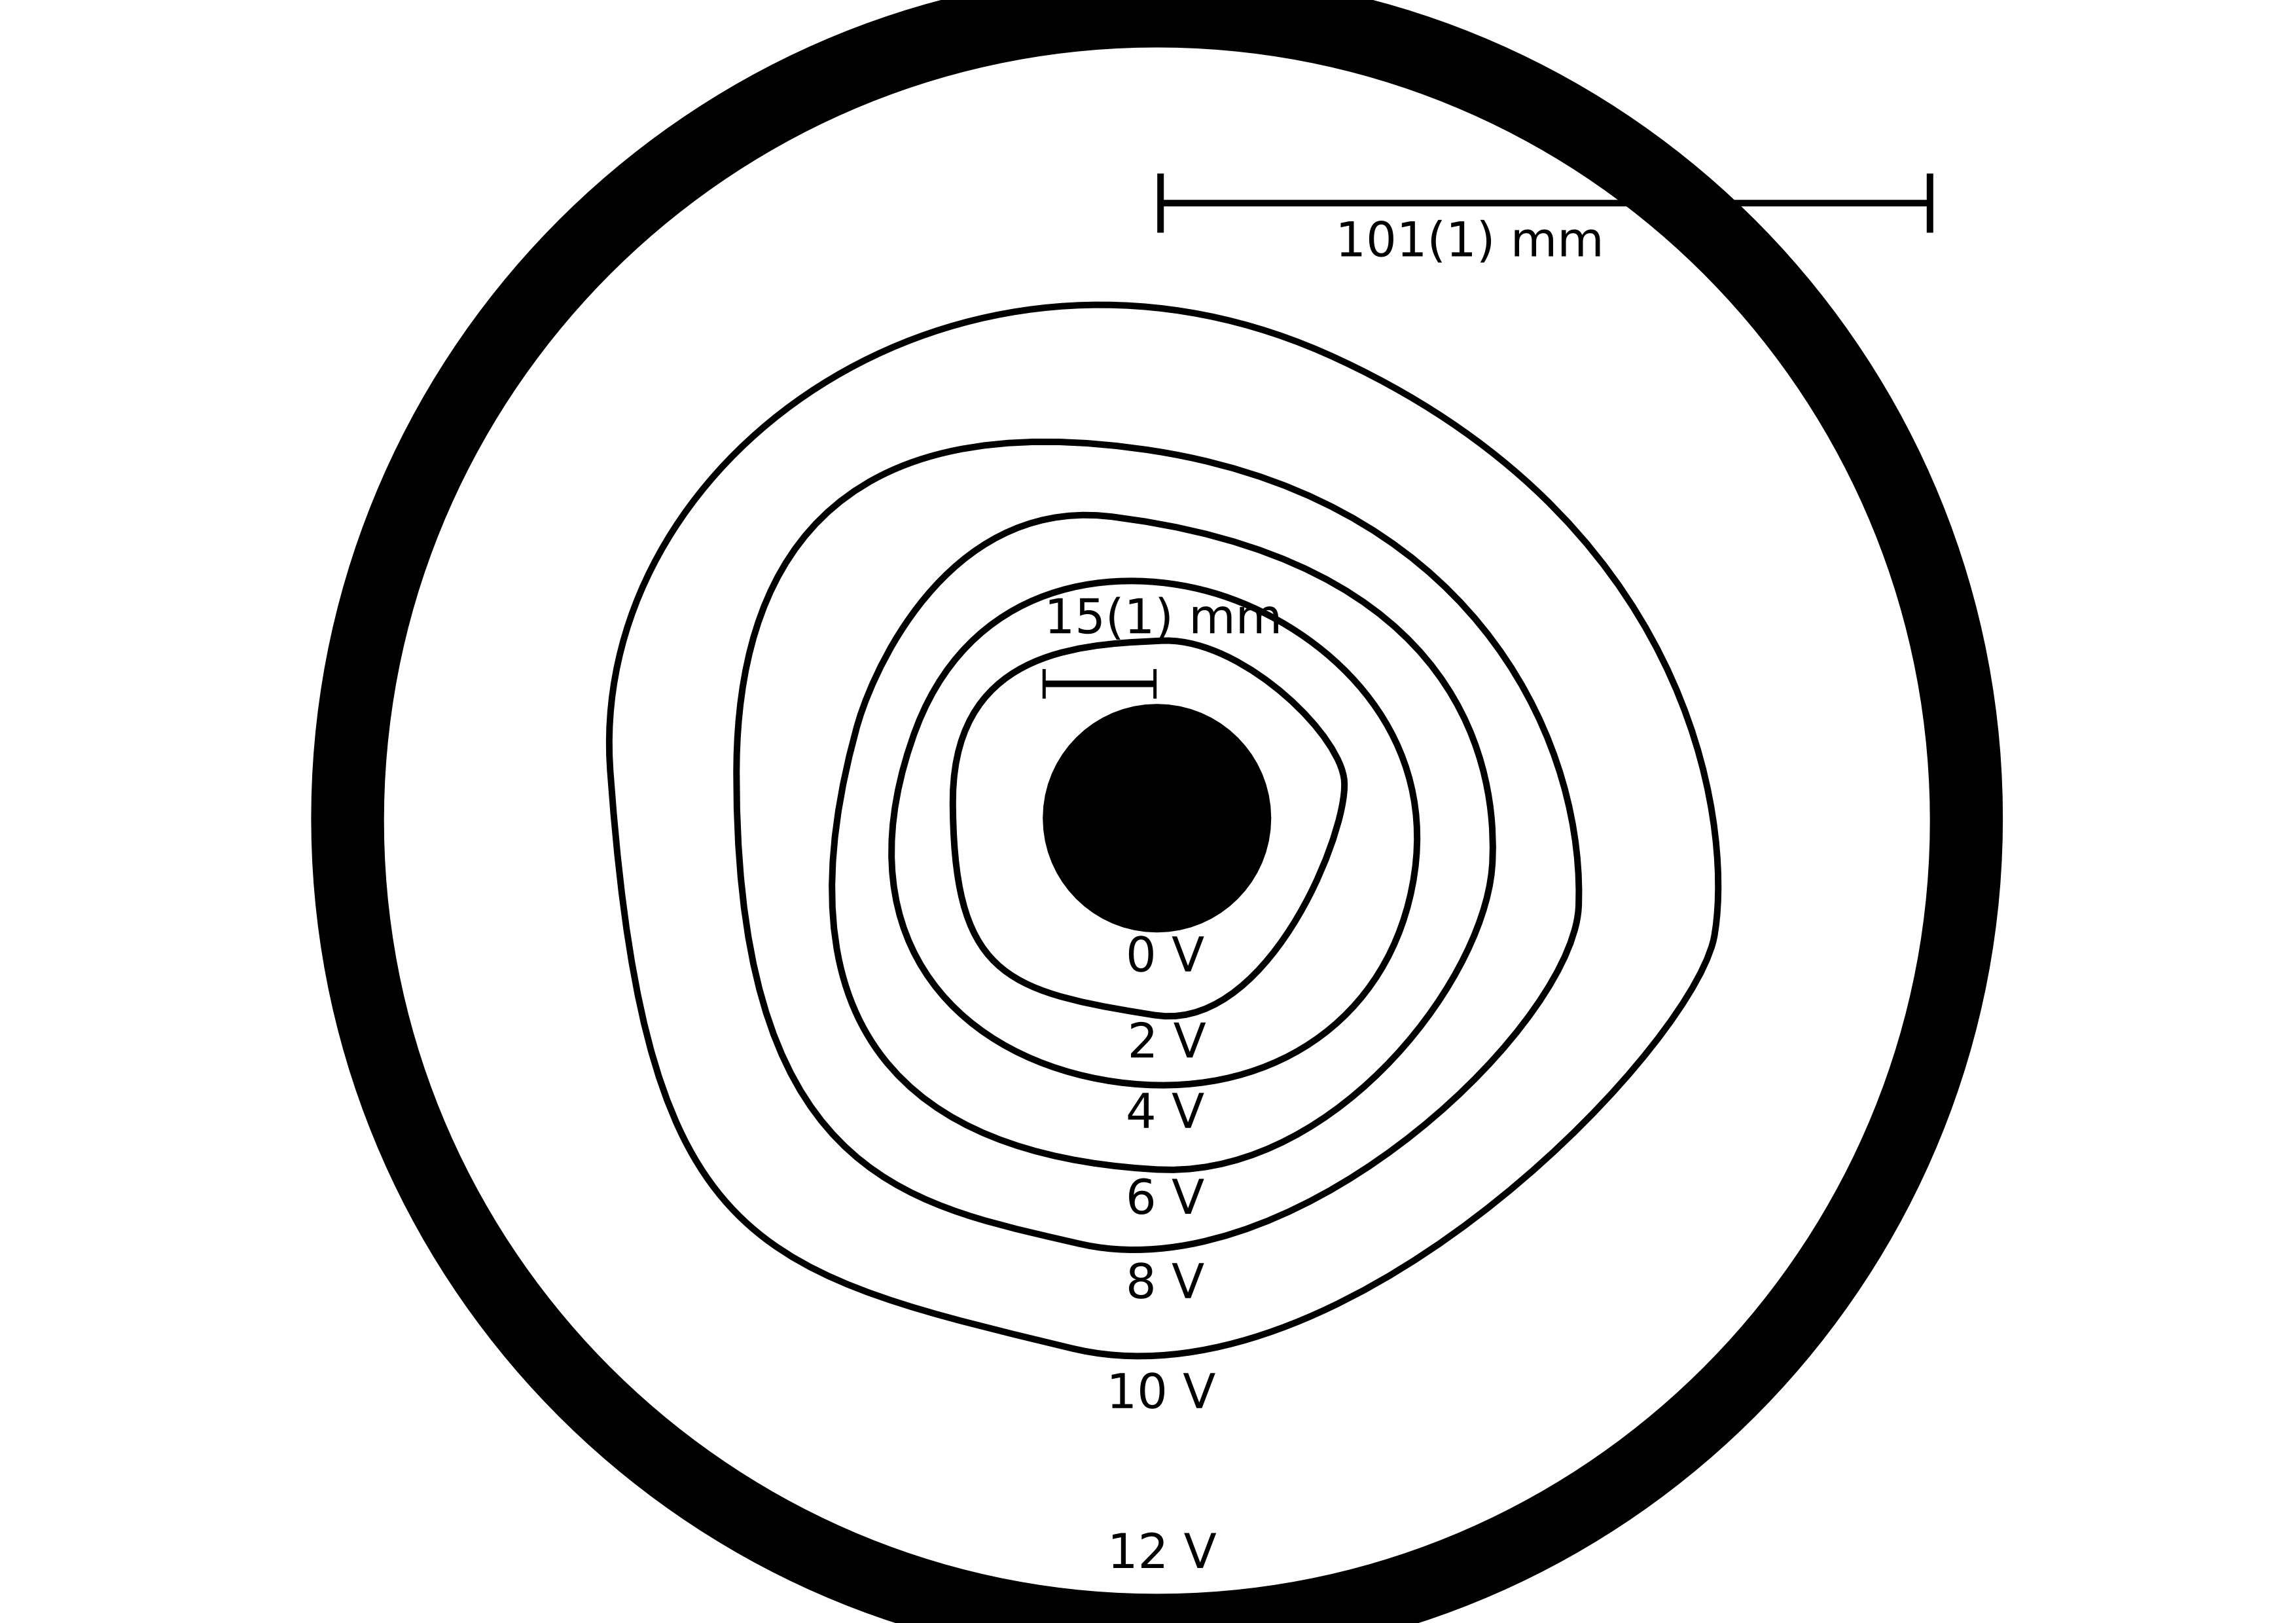
\includegraphics[width = 15cm]{lab2_concentric_cylinders.png}
    \caption{Equipotential lines for the two concentric cylinders}
    \label{fig:concentric_cylinders}
\end{figure}
\begin{figure}
    \centering
    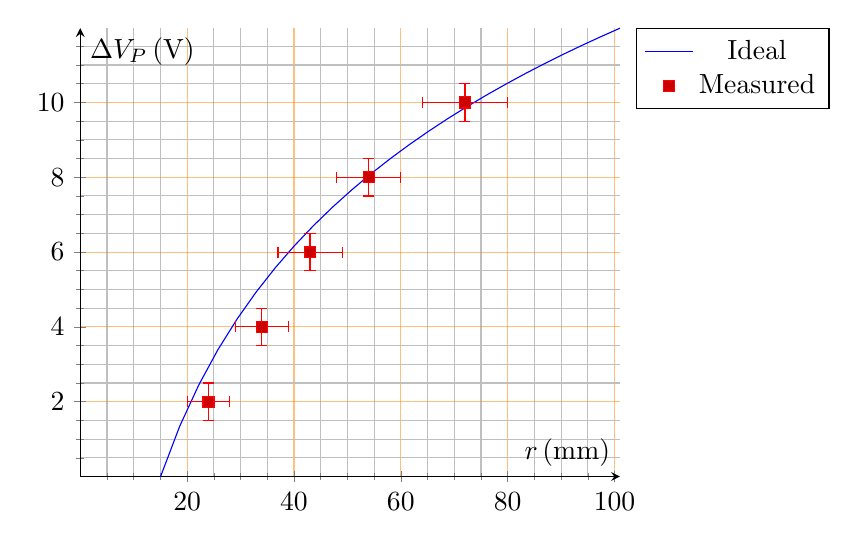
\begin{tikzpicture}
        \begin{axis}[
            potential,
            xlabel = \(r\,\mathrm{(mm)}\),
            ylabel = \(\Delta V_P\,\mathrm{(V)}\),
            xmax = 101
        ]
            \addplot +[no marks, domain = 15:101] {6.29 * (ln(x) - 2.71};
            \addlegendentry{Ideal}
            
            \addplot +[potential-scatter] table [
                x error = xerror,
                y error = yerror
            ] {
                x   y   xerror  yerror
                24  2   4       0.5
                34  4   5       0.5
                43  6   6       0.5
                54  8   6       0.5
                72  10  8       0.5
            };
            \addlegendentry{Measured}
        \end{axis}
    \end{tikzpicture}
    \caption{Voltage difference between the concentric cylinders}
    \label{fig:concentric_cylinders_voltage}
\end{figure}

Figure \ref{fig:concentric_cylinders} shows the equipotential contours recorded. Figure \ref{fig:concentric_cylinders_voltage} shows the measured voltage at radial distances from the axis of the system.

While the measurements fit, within error, to the ideal model, the data gathered was not very precise, with each equipotential line varying significantly in radial distance.

Measurement of the voltage outside of the outer cylinder was also taken, but it was consistently \SI{0.00 \pm 0.01}{\volt}.

\subsection{Separated Parallel Cylinders}
\begin{figure}
    \centering
    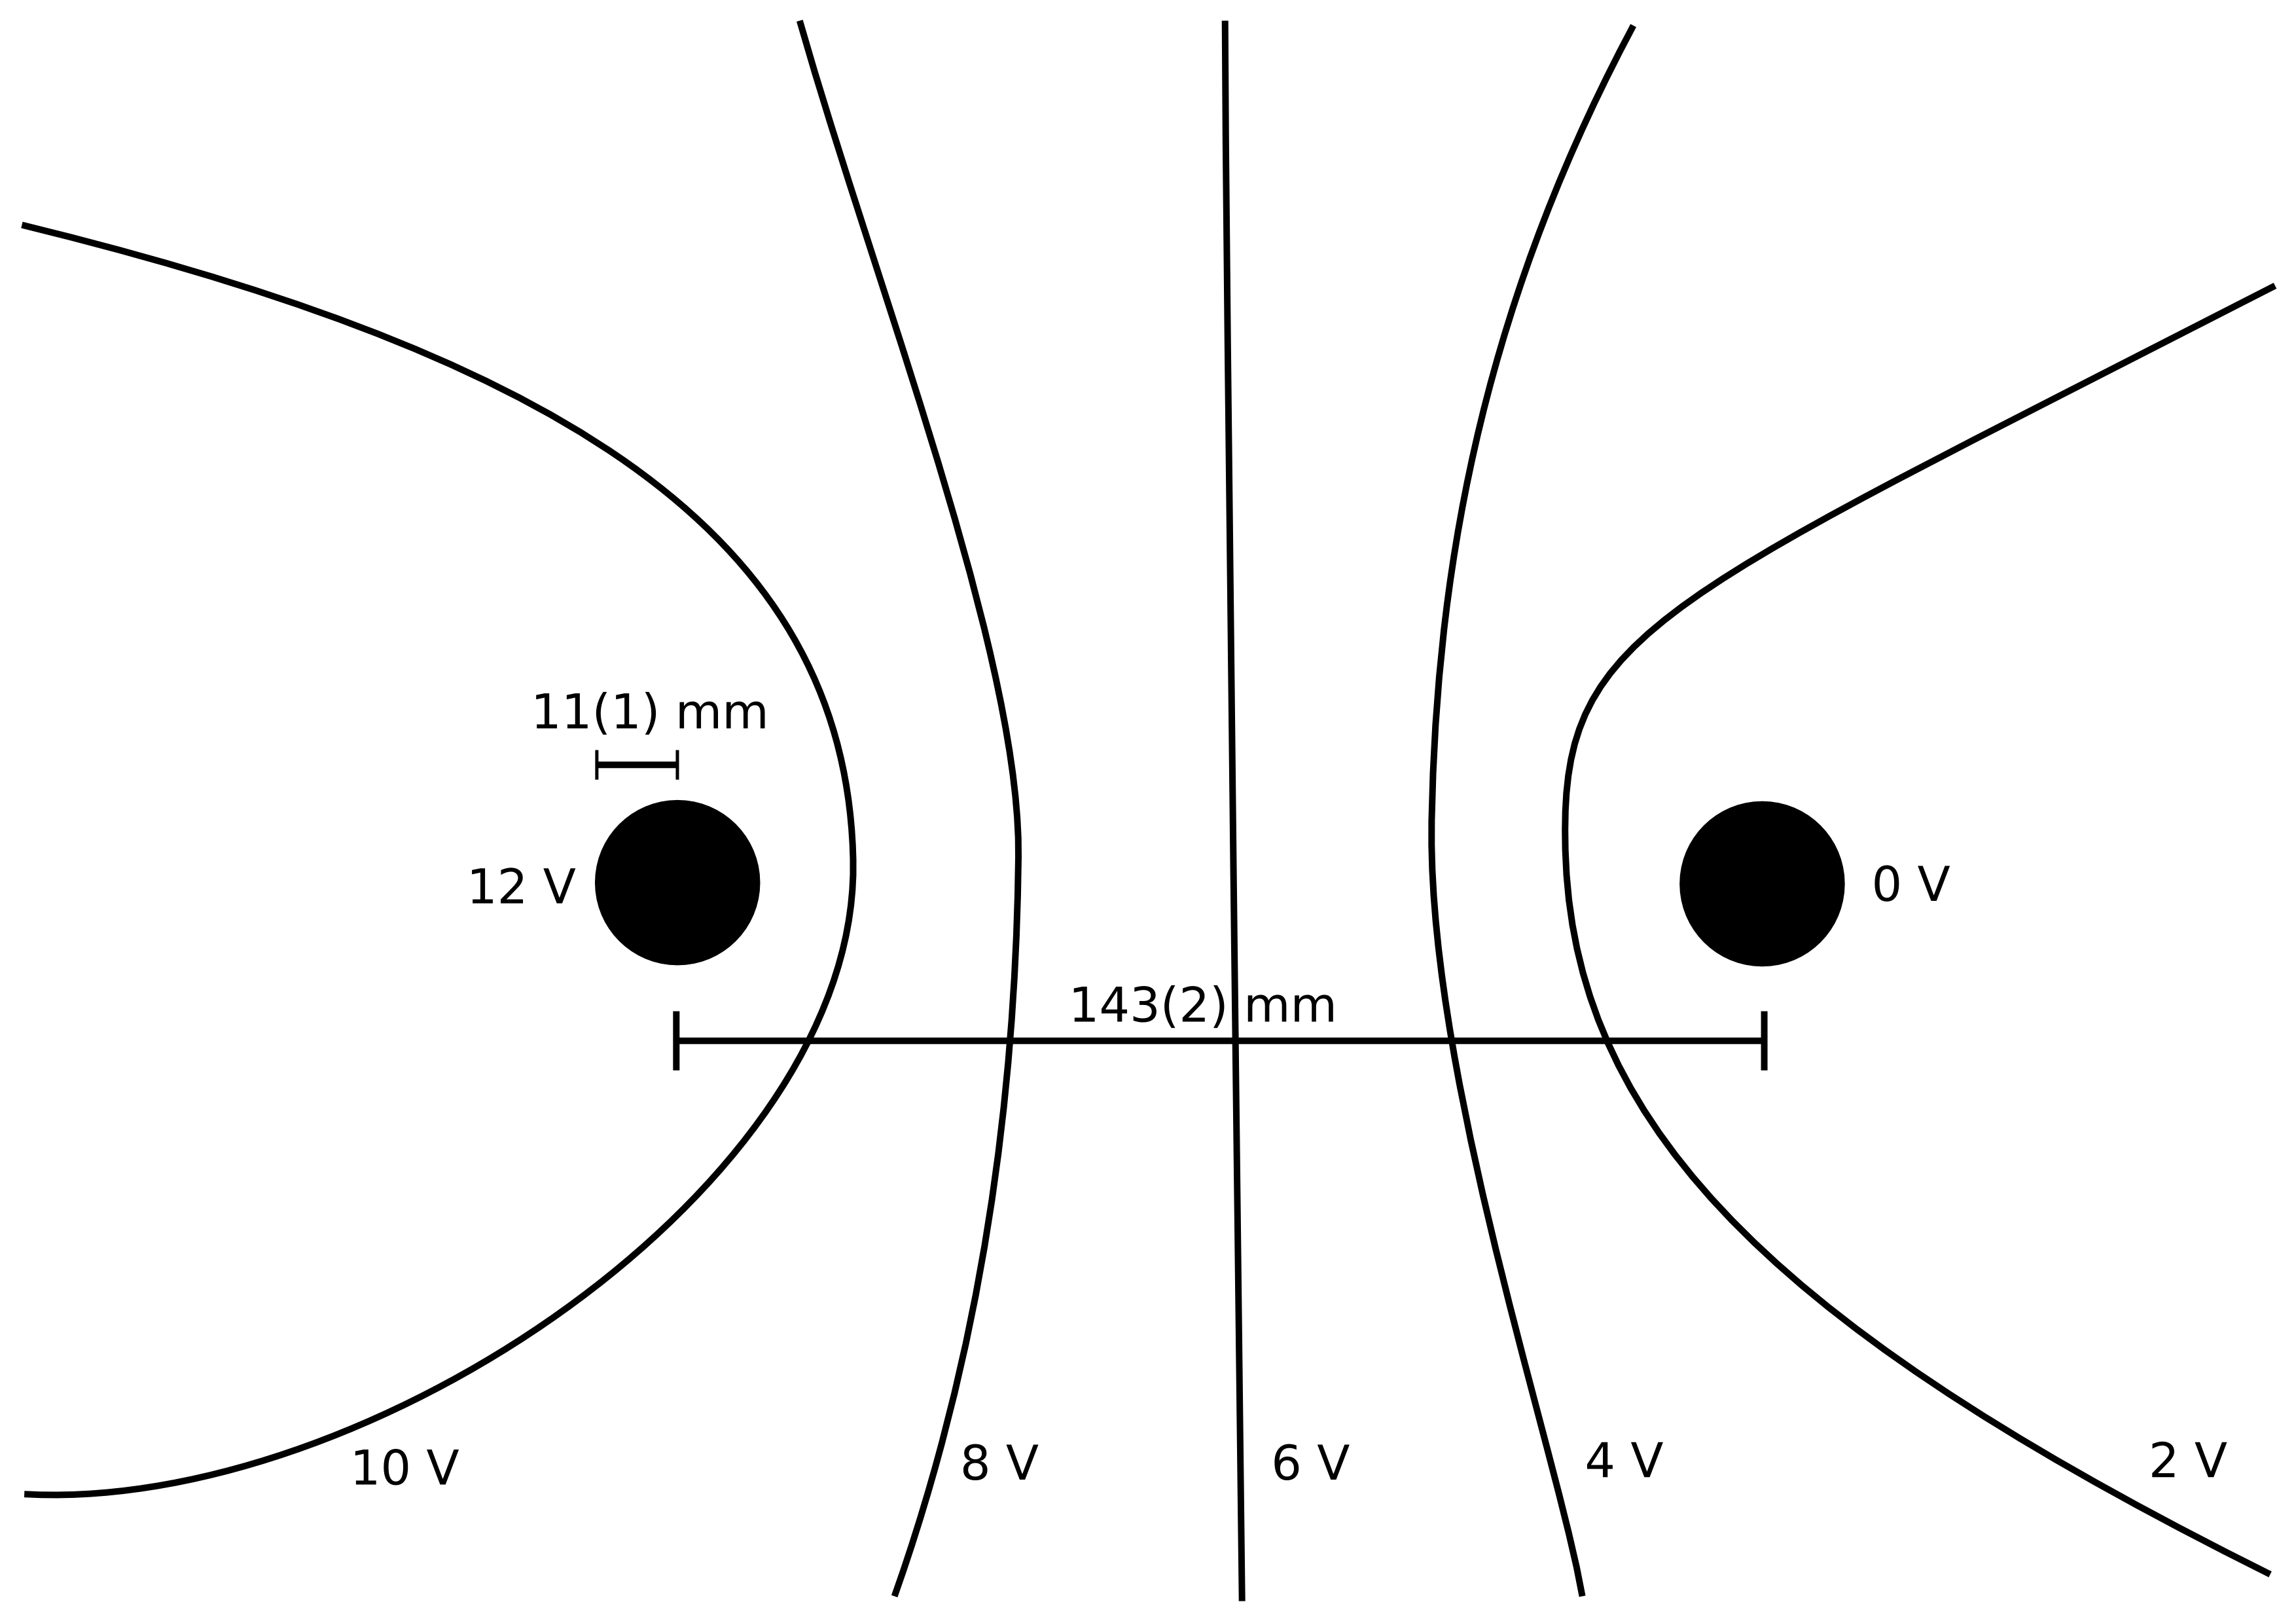
\includegraphics[width = 15cm]{lab2_separated_parallel_cylinders.png}
    \caption{Equipotential lines for the two separated cylinders}
    \label{fig:separated_parallel_cylinders}
\end{figure}
\begin{figure}
    \centering
    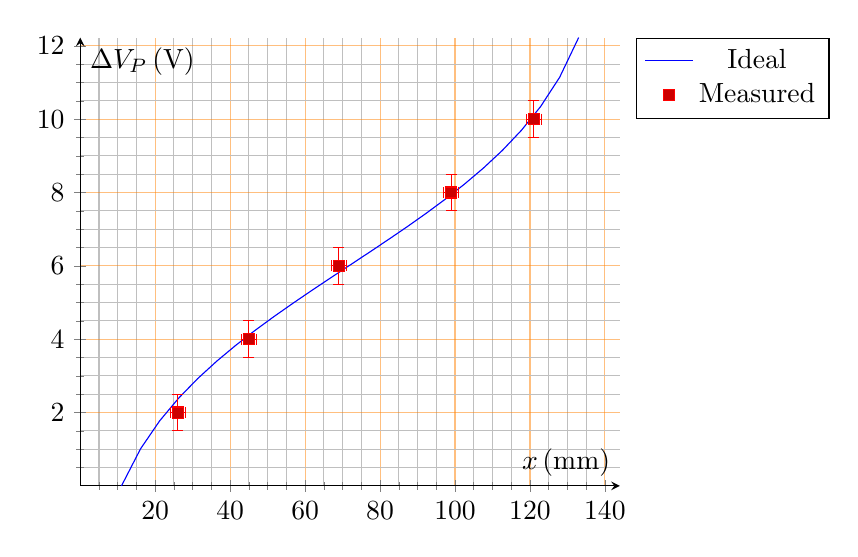
\begin{tikzpicture}
        \begin{axis}[
            potential,
            xlabel = \(x\,\mathrm{(mm)}\),
            ylabel = \(\Delta V_P\,\mathrm{(V)}\),
            xmax = 144
        ]
            \addplot +[no marks, domain = 11:133] {2.41 * ln(12 * x / (143 - x))};
            \addlegendentry{Ideal}
            
            \addplot +[potential-scatter] table [
                x error = xerror,
                y error = yerror
            ] {
                x   y   xerror  yerror
                26  2   2       0.5
                45  4   2       0.5
                69  6   2       0.5
                99  8   2       0.5
                121 10  2       0.5
            };
            \addlegendentry{Measured}
        \end{axis}
    \end{tikzpicture}
    \caption{Voltage difference between the separated cylinders}
    \label{fig:separated_parallel_cylinders_voltage}
\end{figure}

Figure \ref{fig:separated_parallel_cylinders} shows the equipotential contours recorded. Figure \ref{fig:separated_parallel_cylinders_voltage} shows the measured voltage at certain distances along the line through the axes of both cylinders.

The measured values matches the predicted values to well within the error margin.

\section{Discussion}
Most of the data matched the theoretical ideal model within error, suggesting it is reasonably correct in the context of this experiment. Additionally, the measurement of \SI{0.00 \pm 0.01}{\volt} outside of the concentric cylinders also supports the theory.

Most notably of the data that did not fit the ideal model was the bulging of the edge data in figure \ref{fig:parallel_plates_voltage}, which likely is due to edge effects unaccounted for in the model.

The remaining data points that did not fit were very close to fitting, suggesting either impurities in the paper skewing the measurement, or inherent sampling error due to the low number of samples taken. This would especially likely be the case for the concentric cylinder measurements shown in figure \ref{fig:concentric_cylinders_voltage}.

The brief use of the multimeter resulting in the \SI{\pm 3}{\volt} difference indicates a good possibility that the relatively low impedance of the multimeter was causing the inaccurate result.

\end{document}